\chapter{Begrifflichkeit und computergrafische Grundlagen}
\label{CHAP:FUNDAMENTALS}

Bevor die Bewertungskriterien der späteren Evaluation spezifiert werden, sollen zunächst einige häufig vorkommende Fachbegriffe und elementare Konzepte der Computergrafik erläutert werden, um das Verständnis der weiteren Ausführungen zu erleichtern.

\section{Grundbegriffe}
\label{SEC:BASIC_CONCEPTS}

Ein durch das \emph{World Wide Web Consortium} (W3C) definierter Standard für den Zugriff und die Manipulation von HTML- und XML-Dokumenten ist das \textbf{Document Object Model} (DOM). Die durch diese Spezifikation definierte Programmierschnittstelle ermöglicht das Traversieren, Hinzufügen, Ändern und Entfernen von DOM-Elementen, sodass ein Dokument vollständig dynamisch bearbeitet werden kann \autocite{W3C_DOM_CORE_3}. Das World Wide Web Consortium ist ein internationales Gremium zur Standardisierung von Techniken rund um das WWW \autocite{W3C_ABOUT}.

Ein Sammelbegriff für sämtliche Technologien rund um die Darstellung von 3D-""Computergrafik im World Wide Web ist \textbf{Web3D}. Dieses beinhaltet sowohl traditionelle Ansätze auf Basis von Browser-Plugins als auch jüngst aufgekommene native Umsetzungen.
Die Bildsynthese -- oder gängiger: das \textbf{Rendering} -- bezeichnet die Erzeugung eines zweidimensionalen Einzelbilds, welches ausgehend von einer virtuellen 3D-""Darstellung berechnet wird. Dieses Bild kann im Anschluss auf dem Bildschirm oder einem anderen Ausgabemedium angezeigt werden.

\begin{figure}[htb]
	\centering
	\subfloat[Polygonnetz]{
		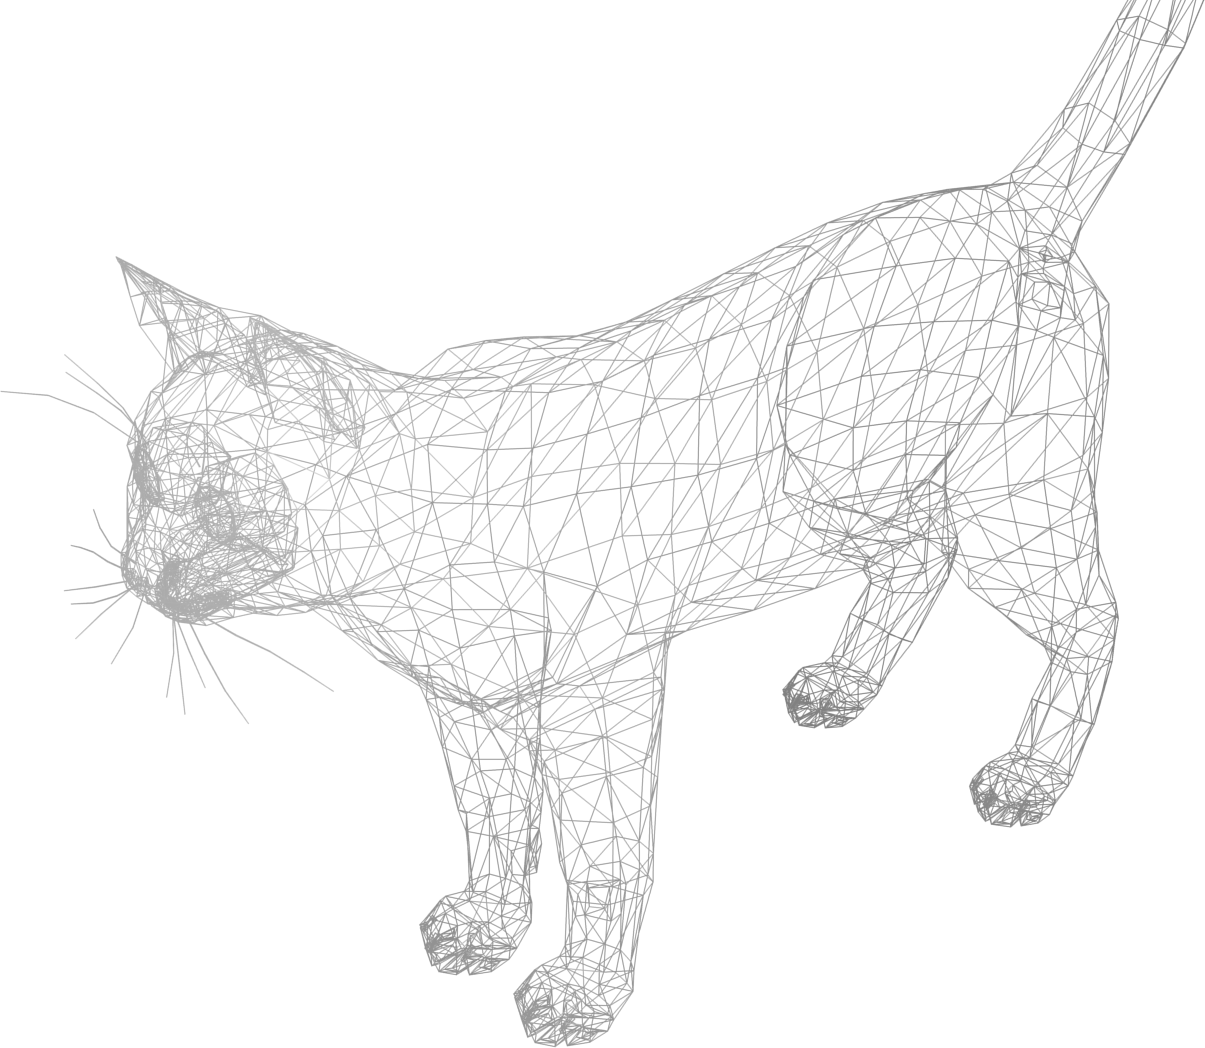
\includegraphics[width=0.31\textwidth]{kap2/figures/cat-wireframe.png}
		\label{FIG:3DMODEL_WIREFRAME}
	}
	\hfill
	\subfloat[Flat-Shading]{
		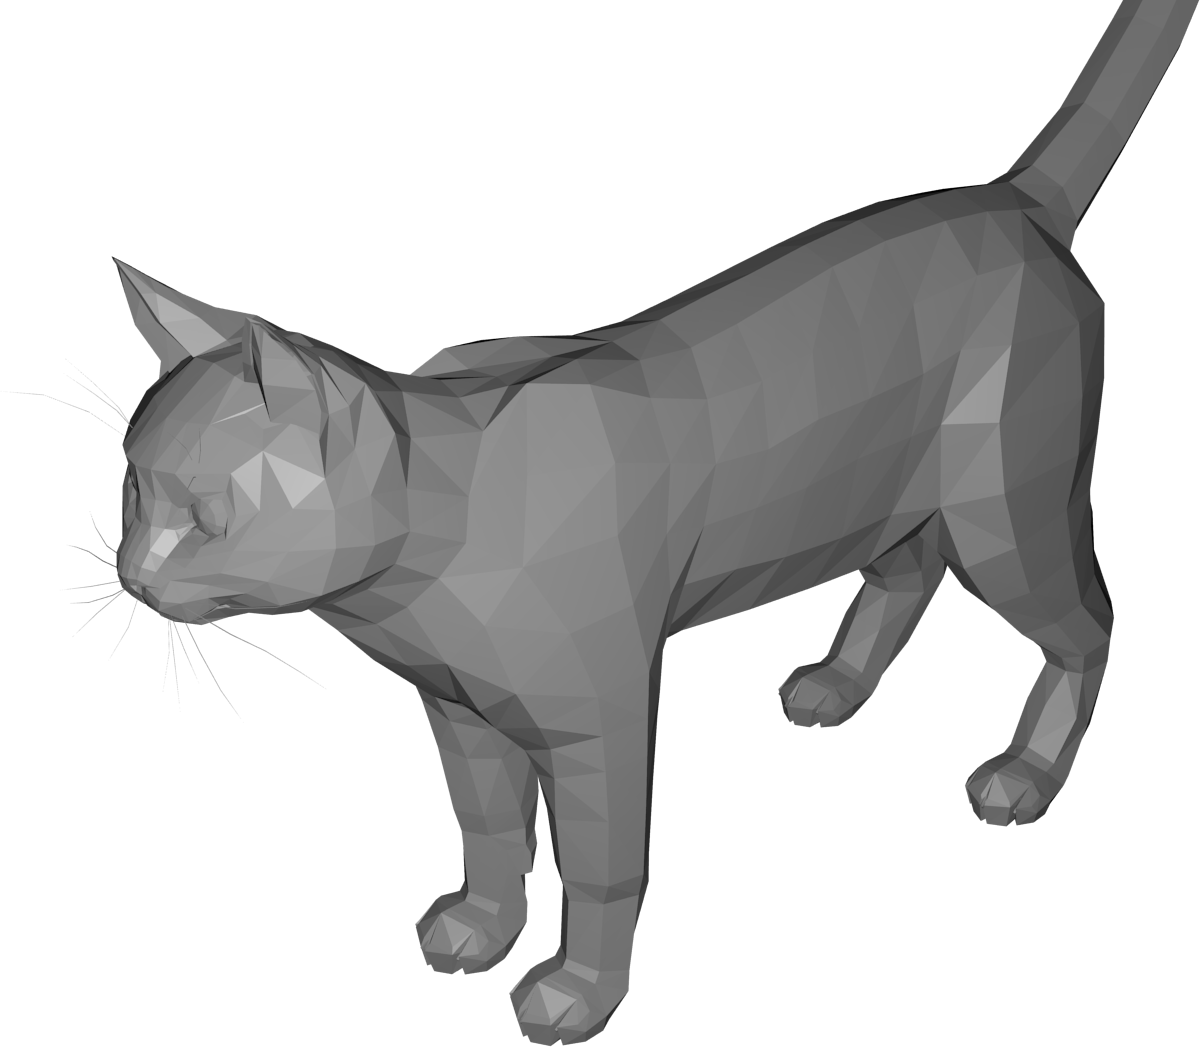
\includegraphics[width=0.31\textwidth]{kap2/figures/cat-flat-shading.png}
		\label{FIG:3DMODEL_FLAT_SHADING}
	}
	\hfill
	\subfloat[Smooth-Shading]{
		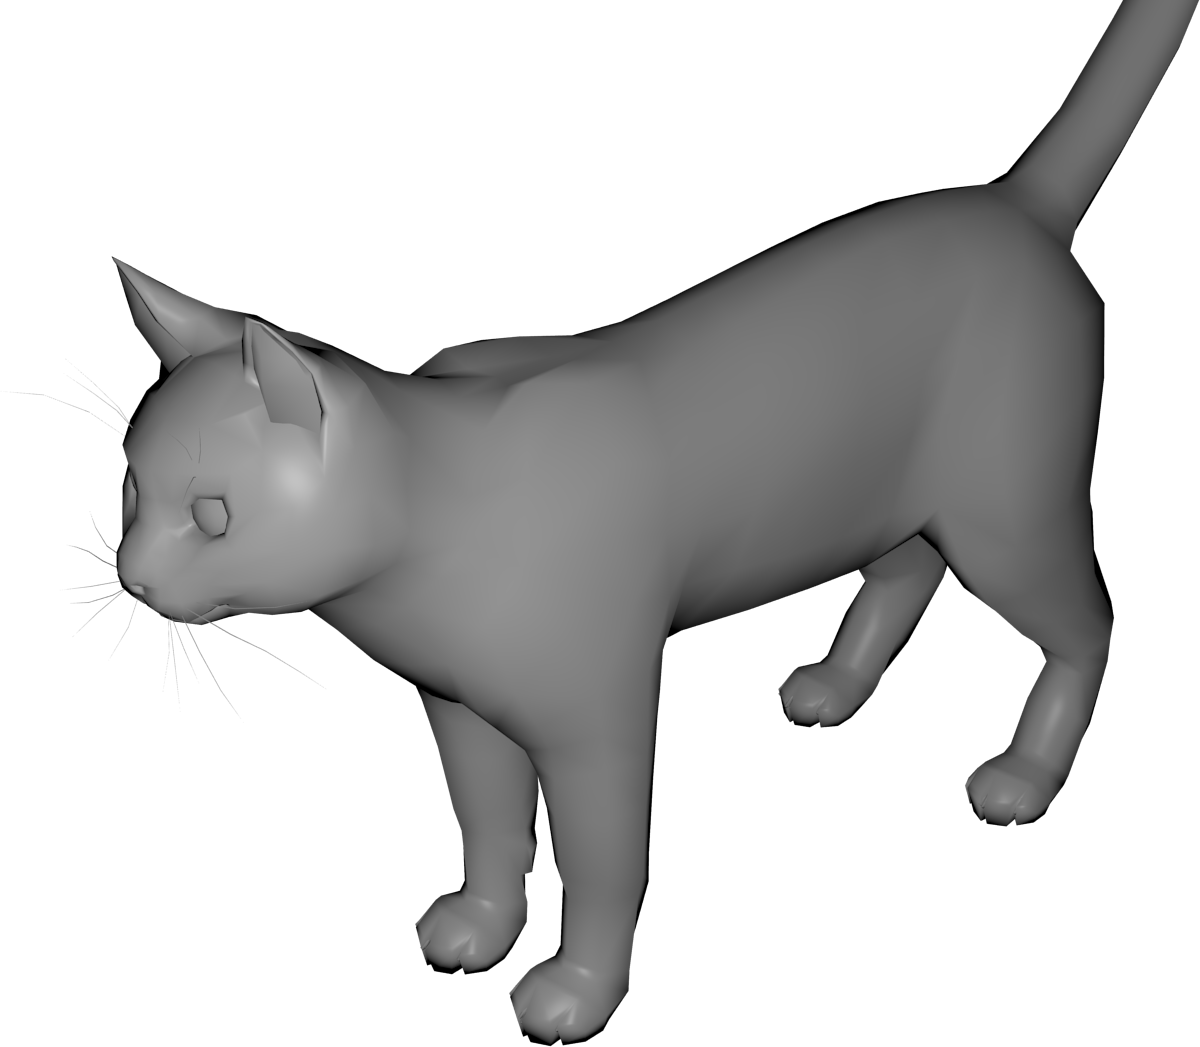
\includegraphics[width=0.31\textwidth]{kap2/figures/cat-smooth-shading-lambert-phong.png}
		\label{FIG:3DMODEL_SMOOTH_SHADING}
	}
	\caption{Verschiedene Darstellungen eines 3D-Modells.}
	\label{FIG:3DMODELS_SHADING}
\end{figure}

Abbildung \ref{FIG:3DMODELS_SHADING} zeigt verschiedene Darstellungen eines \textbf{3D-""Modells}. Ein solches Modell ist die mathematische Repräsentation eines dreidimensionales Objekts im Raum, definiert durch eine Menge von Punkten (\textbf{Vertices}\footnote{Singular: Vertex.}) Kanten. Wie die linke Figur zeigt, verbinden Kanten die Vertices zu einem Polygonnetz, welches die Seiten (\emph{Faces}) des Objekts formt. Als Polygone dienen in der Computergrafik typischerweise Dreiecke. Diese sind aufgrund der Eigenschaft dass sie stets planar vorliegen, besonders gut für grafische Berechnungen geeignet \autocite{MOZILLA_CONCEPTS_OF_WEBGL}. Weiterhin wird die Orientierung der Polygone durch deren Normalenvektor festgelegt. Diese ist zum einen für Sichtbarkeitsentscheide (\emph{Culling}) wichtig und dient zum anderen der Berechnung von Beleuchtungsmodellen. Unter \textbf{Culling} wird eine Reihe von Algorithmen verstanden, die darüber entscheiden, welche Objekte einer 3D-Szene zu zeichnen sind und welche nicht. Elemente, die komplett außerhalb des sichtbaren Bereichs liegen, müssen beispielsweise nicht betrachtet werden und verursachen so keinen unnötigen Rechenaufwand.

Ein \textbf{Beleuchtungsmodell} stellt das Verfahren dar, welches den Einfluss von Licht in einer 3D-Szene simuliert \autocite[190\psq]{Zeppenfeld:2004}. Hierbei wird zwischen dem lokalen und globalen Beleuchtungsmodell unterschieden. Während Ersteres lediglich den Einfluss der Lichtquellen in einem Punkt der Objektoberfläche berücksichtigt, werden beim globalen Modell auch Reflexion, Transparenzeffekte und Lichtbrechung mit einbezogen.

\begin{figure}[ht]
	\centering
	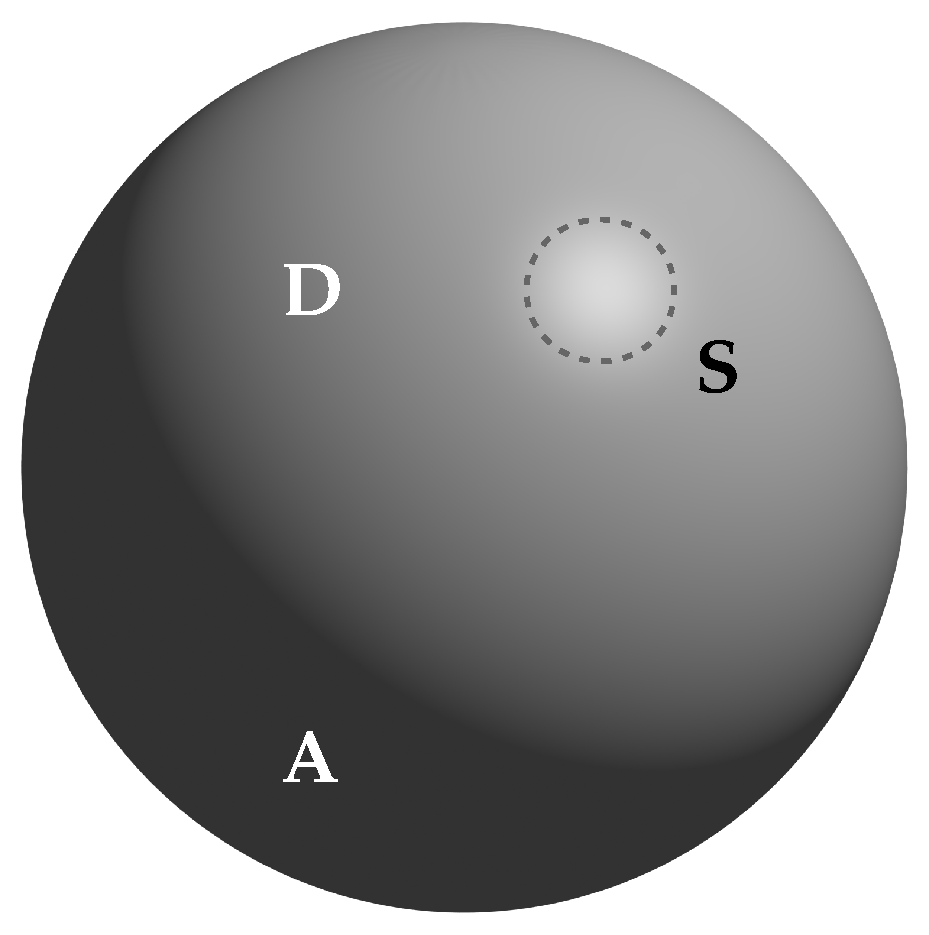
\includegraphics[width=0.25\textwidth]{kap2/figures/illumination-crop.pdf}
	\caption{Ambiente, diffuse und spekulare Beleuchtung.}
	\label{FIG:ILLUMINATION}
\end{figure}

Abbildung \ref{FIG:ILLUMINATION} zeigt wichtige Licht- und Reflexionsmodelle der Computergrafik \autocite[722\psq]{Foley:CG_PRINCIPLES_AND_PRACTICE}. Ambientes Licht (A) kommt aus allen Richtungen und hat somit auf alle Objekte denselben Einfluss, unabhängig von deren Position im Raum. Es sorgt für die Grundhelligkeit einer Szene, sodass selbst im Schatten liegende Objekte nicht tiefschwarz sind, sondern eine Grauschattierung aufweisen. Die diffuse Reflexion (D) führt zu einer gleichmäßigen Reflexion des Lichts in alle Richtungen. Da der Einfallswinkel des Lichts hierbei berücksichtig wird, entsteht ein plastischer Eindruck. Die spekulare oder spiegelnde Reflexion (S) sorgt schließlich für Glanzeffekte (\emph{Highlights}) auf der Materialoberfläche.

Die Abbildungen \ref{FIG:3DMODEL_FLAT_SHADING} und \ref{FIG:3DMODEL_SMOOTH_SHADING} auf der vorherigen Seite zeigen verschiedene Schattierungsverfahren (\textbf{Shading}). Der weit gefasste Begriff \emph{Shading} bezeichnet die Berechnung der Beleuchtung und Materialeigenschaften von Objektoberflächen. Durch Anwendung von \emph{Flat-Shading} (Mitte) wird die Farbe jedes Polygons durch dessen Normale entsprechend des lokalen Beleuchtungsmodells berechnet. Hieraus resultiert eine einheitliche Färbung des gesamten Polygons. Das \emph{Smooth-Shading} (rechts) -- genauer ein sogenanntes \emph{Phong-Shading}\footnote{Benannt nach Erfinder des Verfahrens, dem vietnamesischen Computergrafiker Bui Tuong Phong.} -- führt zu einer glatten Oberfläche, indem die Normalen der Polygone interpoliert werden und die Farbe jedes Pixels hiervon ausgehend erneut durch Anwendung des lokalen Beleuchtungsmodells berechnet wird \autocite[203\psq]{Zeppenfeld:2004}. Das Phong-Verfahren erzeugt weiterhin Glanzeffekte durch spekulare Reflexion (siehe Kopf der Katze in Abbildung \ref{FIG:3DMODEL_SMOOTH_SHADING}).

\begin{figure}[ht]
	\centering
	\small
	\Tree [.{\textbf{Universum}} Lichtquelle [.{Affine Transformation} [.{Modell 1} Geometrie Material ] {Modell 2} ] ]
	\caption{Exemplarischer Szenengraph (unvollständig).}
	\label{FIG:SCENEGRAPH_EXAMPLE}
\end{figure}

Eine in der Computergrafik häufig vorkommende Datenstruktur zur Repräsentation hierarchischer 3D-""Szenen ist der sogenannte \textbf{Szenengraph}. Hierbei handelt es sich um einen gerichteten azyklischen Graph, dessen Wurzelknoten das \emph{Universum}, also die vollständige Szene darstellt. Kindknoten der Wurzel sind Objekte der Szene und können wiederum weitere Elemente enthalten (vgl. Abbildung \ref{FIG:SCENEGRAPH_EXAMPLE}). Transformationen auf einen Knoten werden auf alle Kinder weitervererbt.

\section{Standard-Grafikpipeline}
\label{SEC:STANDARD_GRAPHICS_PIPELINE}

Ein weiteres elementares Konzept nahezu aller heutigen Grafiksysteme ist die sogenannte Grafik- oder Rendering-Pipeline \cite[866-871]{Foley:CG_PRINCIPLES_AND_PRACTICE}. Diese beschreibt die Gesamtheit der Einzelschritte, die nötig sind, um eine virtuelle 3D-""Szene mittels mehrerer Transformationen und Berechnungen auf den zweidimensionalen Bildschirm abzubilden. Die späteren Beispiele der betrachteten Technologien werden diese Konzepte praktisch widerspiegeln.

Der Begriff \enquote{Pipeline} kann analog zu klassischen UNIX-Pipelines gesehen werden und verdeutlicht das Prinzip des Verfahrens: Die Ausgabe einer Operation dient als Eingabe des nächsten Prozesses.
Die Effizienz der grafischen Berechnungen wird hierbei wie in Abbildung \ref{FIG:RENDERING_PIPELINE} angedeutet durch Parallelisierung innerhalb des Grafikprozessors (\emph{Graphics Processing Unit}), dessen Hardware hinsichtlich dieser Anforderung optimiert ist, enorm gesteigert. Vor jedem Schritt muss die Pipeline auf Fertigstellung der vorherigen Berechnung warten. Abbildung \ref{FIG:RENDERING_PIPELINE} zeigt den schematischen Aufbau der Pipeline:

\begin{figure}[hb]
	\centering
	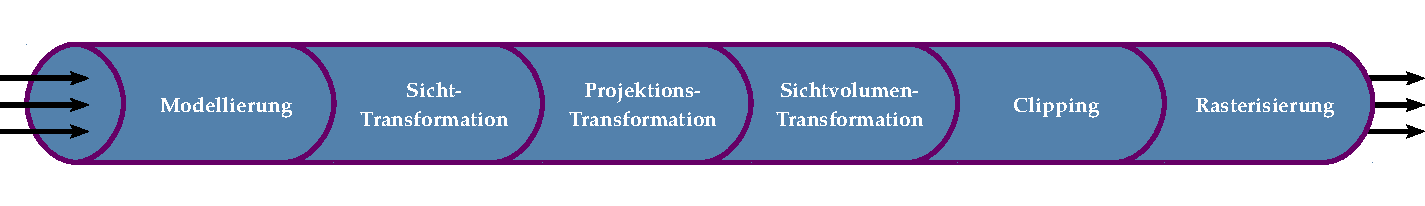
\includegraphics[width=1.0\textwidth]{kap2/figures/rendering-pipeline-crop.pdf}
	\caption{Schematische Darstellung der Standard-Grafikpipeline.}
	\label{FIG:RENDERING_PIPELINE}
\end{figure}

Während die Funktionalität der Pipeline zu Anfang der Hardware-""Entwicklung statisch umgesetzt war (\emph{Fixed-Function-Pipeline}) und nur durch wenige Parameter angepasst werden konnte, sind heutige Implementierungen durch sogenannte \emph{Shader} vollständig programmierbar und weisen eine hohe Flexiblität auf\footnote{Shader-Programme werden in Abschnitt \ref{SEC:WEBGL_SHADER} näher behandelt.}. Die Grafikpipeline kann sowohl in Hardware als auch in Software umgesetzt werden. Hardware-""Implementierungen sind Software-basierten Realisierungen jedoch hinsichtlich der Effizienz und Geschwindigkeit deutlich überlegen und daher zu bevorzugen.

Im Folgenden werden die Einzelschritte der Pipeline erläutert. Die Details der konkreten mathematischen Berechnungen werden hierbei nicht weiter ausgeführt, da sie den Rahmen der vorliegenden Arbeit übersteigen.

\subsection{Modellierung}
Zu Beginn des Verfahrens steht das Laden beziehungsweise die Konstruktion der 3D-Modelle.
Nach der Definition von Eckpunkten (\emph{Vertices}) durch Angabe derer kartesischer Koordinaten werden die Modelle durch Polygone zusammengesetzt. Als Polygone dienen typischerweise Dreiecke aufgrund der bereits genannten Vorteile. Diese werden durch je drei Vertices definiert. Natürlich ist eine manuelle Definition der Geometrie in realen Anwendungsfällen bei komplexen Modellen mit zehntausenden von Vertices ausgeschlossen. Gemeinhin enstammen die geometrischen Daten spezieller 3D-""Model"-lierungs"-software wie \emph{Blender} \autocite{SOFTWARE_BLENDER}, die die Erstellung aufwendiger Modelle erheblich erleichtern.

Die Koordinaten der Vertices liegen zunächst relativ zur \enquote{Modelmitte} in einem lokalen Koordinatensystem vor. Mittels affiner Transformationen können die Modelle im Raum verschoben, skaliert, rotiert und verzerrt werden. Dies wird durch Multiplikation der entsprechenden, homogenen Transformationsmatrix mit allen Punkten des Modells realisiert. Weiterhin können mehrere Transformationen durch Multiplikationen aller beteiligten Matrizen durch eine einzige gleichwertige Modellmatrix $\underline{M}$ ersetzt werden. Da die Matrizenmultiplikation nicht kommutativ ist, ist die Reihenfolge der Operation entscheidend.

Eine Überführung der Modelkoordinaten in sogenannte Weltkoordinaten wird somit durch folgende Berechnung vollzogen. Dabei sei $\vec{v}_i$ der Spaltenvektor der Koordinaten des aktuell betrachteten Vertex.

\begin{figure}[!h]
	\begin{displaymath}
		\sum_{i=0}^{n} \underline{M} * \vec{v}_i
	\end{displaymath}
	\caption{Berechnung der Modelmatrix.}
\end{figure}

\subsection{Sicht-Transformation}

Anschließend wird die Ansicht der Szene mittels mehrerer Parameter festgelegt. Der Aug- oder Beobachtungspunkt, welcher der \enquote{Kamera} der Szene entspricht, wird zunächst im Weltkoordinatensystem platziert. Des Weiteren wird das Zentrum der Betrachtung der (\emph{Look-At}-Punkt) und der Oben-Vektor spezifiziert. Dieser legt die Orientierung der Ansicht fest, indem er die Richtung \enquote{oben} definiert.

All diese Parameter werden innerhalb der Sichtmatrix $\underline{V}$ abgebildet. Durch Multiplikation der Modellmatrix und der Vertices mit der Sichtmatrix erfolgt die Transformation in das sogenannte Sichtkoordinatensystem. Die Welt wird hierdurch relativ zur Kamera verschoben, welche nun im Ursprung liegt.

\begin{figure}[!h]
	\begin{displaymath}
		\sum_{i=0}^{n} \underline{V} * \underline{M} * \vec{v}_i
	\end{displaymath}
	\caption{Berechnung der MV-Matrix.}
\end{figure}

\subsection{Projektions- und Sichtvolumen-Transformation}
Der nächste Schritt ist die Projektion der Darstellung auf einen Einheitswürfel zur Vorbereitung der Bildschirm-Transformation. Hierfür muss zunächst ein Sichtvolumen definiert werden. Dieses grenzt den darzustellenden Bereichs des 3D-""Raums durch Ebenen ein und wird für das spätere \emph{Clipping} benötigt. Um die Darstellungseffizienz zu steigern, werden dabei Objekte außerhalb dieser Abgrenzung verworfen.

Es stehen verschiedene Projektions-Modelle zur Verfügung. Von besonderer Bedeutung sind die orthogonale Parallelenprojektion und die perspektive Projektion.
Bei der Parallelenprojektion wird das Sichtvolumen durch einen Quader beschrieben, welcher mittels Angabe der Dimensionen für die Ausdehnung des Quaders in alle drei Achsen aufgespannt wird. Die spätere Transformation auf den Einheitswürfel ist in diesem Fall mittels einer Skalierung einfach umzusetzen.
Zur Erzielung eines perspektivischen Effekts, also der Größendarstellung von Objekte in Abhängigkeit von deren Entfernung zum Beobachtungspunkt, wird bei der perspektivischen Projektion ein Pyradmidenstumpf (\emph{Frustum}) verwendet. Durch die verzerrende Abbildung des Frustums auf den Einheitswürfel entsteht so die angestrebte kleinere Darstellung weiter entfernter Elemente.

\begin{figure}[!h]
	\begin{displaymath}
		\sum_{i=0}^{n} \underline{P} * \underline{V} * \underline{M} * \vec{v}_i
	\end{displaymath}
	\caption{Berechnung der MVP-Matrix.}
	\label{CALC:MVP_MATRIX}
\end{figure}

Analog zu den vorherigen Schritten wird auch diese Berechnung durch eine Matrixmultiplikation realisiert. Durch Multiplikation der bisherigen Transformationen mit der Projektionsmatrix, welche die Parameter des gewählten Projektionsmodells enthält, wird hierbei die finale Transformation der Vertices erzielt.

Wie Formel \ref{CALC:MVP_MATRIX} zeigt, kann die gesamte Modell-, Sicht- und Projektionstransformation durch das Matrizenprodukt von $\underline{P}$, $\underline{V}$ und $\underline{M}$ realisiert werden. Dieses Gesamtprodukt der Transformation wird als \emph{MVP-Matrix} bezeichnet. Anstatt für jeden Vertex drei teure Matrizenmultiplikationen durchzuführen, kann die Berechnungseffizienz deutlich gesteigert werden, indem jeder der Punkte lediglich mit der MVP-Matrix multipliziert wird.

\subsection{Clipping}

Nachdem bereits Polygone, welche entweder abgewandt (\emph{Backface-Culling}) oder komplett außerhalb des Sichtvolumens liegen (\emph{Frustum-Culling}\footnote{Bei einer perspektivischen Projektion.}), verworfen wurden, ist der nächste Schritt das sogenannte \emph{Clipping}. Dieses Verfahren betrachtet Polygone, welche das Sichtvolumen schneiden und daher nur teilweise gezeichnet werden müssen. Zu diesem Zweck werden die Schnittpunkte des Polygons mit der Abgrenzung berechnet und anhand dessen ein entsprechendes neues Teilpolygon erstellt. Der Algorithmus von \emph{Cohen-Sutherland} ist ein bekanntes Beispiel für die Realisierung dieses Vorgangs.

Häufig wird dieser Schritt auch der nachfolgenden Rasterisierung zugeordnet. Die Reihenfolge der einzelnen Berechnungen in der Pipeline kann je nach Grafiksystem und Implementierung variieren.

\subsection{Rasterisierung}

Der letzte Schritt der Grafikpipeline ist schließlich die Rasterisierung, welche der finalen Abbildung der 3D-Darstellung auf einzelne Bildpunkte (\emph{Pixel}) dient. Aufgrund des durch die vorherigen Transformationen entstandenen Koordinatensystems in Form eines Einheitswürfels ist eine Abbildung auf die diskreten Abmessungen des Ausgabefensters einfach umzusetzen. Der Rasterisierungs-Prozess kann in zwei Unterpunkte gegeliedert werden:

Zunächst wird mittels eines \emph{Scanline}-Verfahrens eine Verdeckungsberechnung der Polygone durchgeführt. Hierdurch wird bestimmt, welche Punkte der Darstellung zu zeichnen sind und welche nicht, da sie durch Figuren im Vordergrund verdeckt werden. Ein Scanline-Verfahren ist ein Algorithmus, welcher Zeile für Zeile über ein gerastertes Bild iteriert und zu zeichnende Pixel ermittelt. Der zweite Schritt ist anschließend die Einfärbung dieser Pixel durch den in Abschnitt \ref{SEC:BASIC_CONCEPTS} kurz umrissenen Shading-Prozess. Hierbei stehen verschiedene Verfahren wie \emph{Flat-} und \emph{Smooth-Shading} zur Verfügung, welche zu verschiedenen Graden an Realismus und Glattheiten der Oberfläche führen. Ebenso wird hier die Texturierung der 3D-Modelle vorgenommen.
